\chapter{Étude longitudinale sur une maquette à trois degrés de liberté}
\minitoc

\section{Motivation}

\section{Schéma de commande linéaire proportionnel intégral}

\section{Maquette expérimentale}

\section{Test bench presentation}\label{sec:test_bench}
\subsection{Motivation for the design}\label{subsec:motivation}
Closed-loop simulations with the controller developed in \cite[]{sansouECC}, show that in the presence of constant horizontal wind in the $(x_{[B]},z_{[B]})$ plane, the UAV changes its pitch angle. This behaviour has also been observed in wind tunnel tests with the experimental device. Intuitively speaking, a reduced angle of attack leads to a smaller surface area facing the wind, so as to reduce the drag force, which strongly impacts the position. At the same time, the air flow due to the constant wind generates lift, compensated by a reduced propeller thrust and a consequent reduction of the UAV consumption. The goal of the prototype described here is to evaluate experimentally the effect of the wind on the DarkO device.

% \begin{table}[ht]
%   \centering
%     \begin{tabular}{|l|c|c|}
%       \hline
%       \multicolumn{1}{|c|}{Parameter} & Value & Units  \\
%       \hline
%       $m$ (virtual drone mass)  & 0.492 & \SI{}{\kilogram} \\
%       \hline
%       $b$ (wingspan)  & 0.55 & \SI{}{\meter} \\
%       \hline
%       $c$ (aerodynamic cord)  & 0.13 & \SI{}{\meter} \\
%       \hline
%       $S$ (wing area) & 0.0743 & \SI{}{\square\meter}\\
%       \hline
%     \end{tabular}
%     \vspace{0.5cm}
%     \caption{\label{tab:pars} Numerical parameters of the DarkO virtual flight test rig.}
% \end{table}

\subsection{Physical description, sensing, and actuation}

The developed prototype comprises 3D printed parts in Onyx and PLA (polylactic acid, a thermoplastic polyester). It is especially designed for running experiments in front of a wind tunnel with responses that resemble those of the DarkO due to the similar shape (see Fig. \ref{fig:real_test_bench}). The central part, which contains the onboard avionics (autopilot, GPS, etc.) in the DarkO, has been here replaced by a one-degree of freedom revolute joint (see Fig. \ref{fig:rotation}). The wings are the same as those of the DarkO, with the electronic speed controllers (ESC), governing the brushless motor speed, placed in the wings. As described in Section \ref{subsec:motivation}, we wish to represent and study the $y$-axis degree of freedom of the DarkO UAV. The main carbon tube linking the two wings is used as the rotation axis. This tube is fixed to two bearings placed 28.5 mm apart in order to obtain a solid fixation of the rig. This rotation axis is equipped with an optical quadrature rotary encoder to accurately measure the orientation of the device. The advantage of this sensor is that it does not produce torque on the rotation axis. This encoder offers 4000 edges per revolution, which results in a resolution of $0.09^\circ/pulse$.

%TODO modif image plus d'explication
\begin{figure}[!ht]
    \centering
    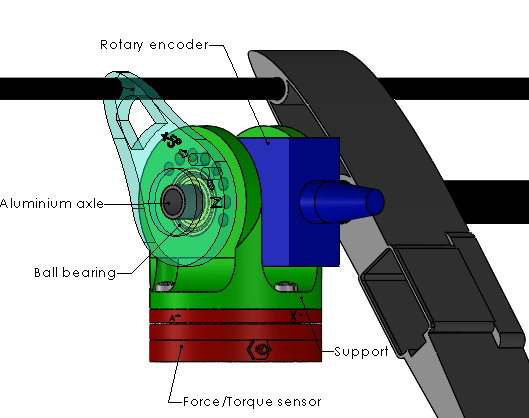
\includegraphics[width=0.8\columnwidth]{figures/MontageSupport2.PNG}
    \caption{The one degree-of-freedom joint.}
    \label{fig:rotation}
\end{figure} 
As shown in Fig. \ref{fig:rotation}, the indexer and the holder are drilled so that the rotation can be locked at known positions ($0^\circ$, $90^\circ$, etc.) by a screw on the indexer that fits into the holes of the holder. Locking the device allows for a correct initialization of the incremental encoder. Locking also allows placing the device in specific exact positions in order to identify the aerodynamic coefficients. 
%TODO Expliquer le roulement, frottement etc

The pivoting joint is also equipped with a 6 degrees of freedom (DOF) force-torque sensor, providing a measurement of the internal wrench exerted on the experimental device by the support. The experimental test bench is also equipped with a hot wire to measure the airspeed seen by the drone. 

% \begin{figure}[!ht]
%         \includegraphics[width=\columnwidth]{picture/Complet.PNG}
%     \caption{Sketch of the developed experimental device in the one DOF configuration.}
%     \label{fig:model}
% \end{figure}\\
\begin{figure}[!ht]
    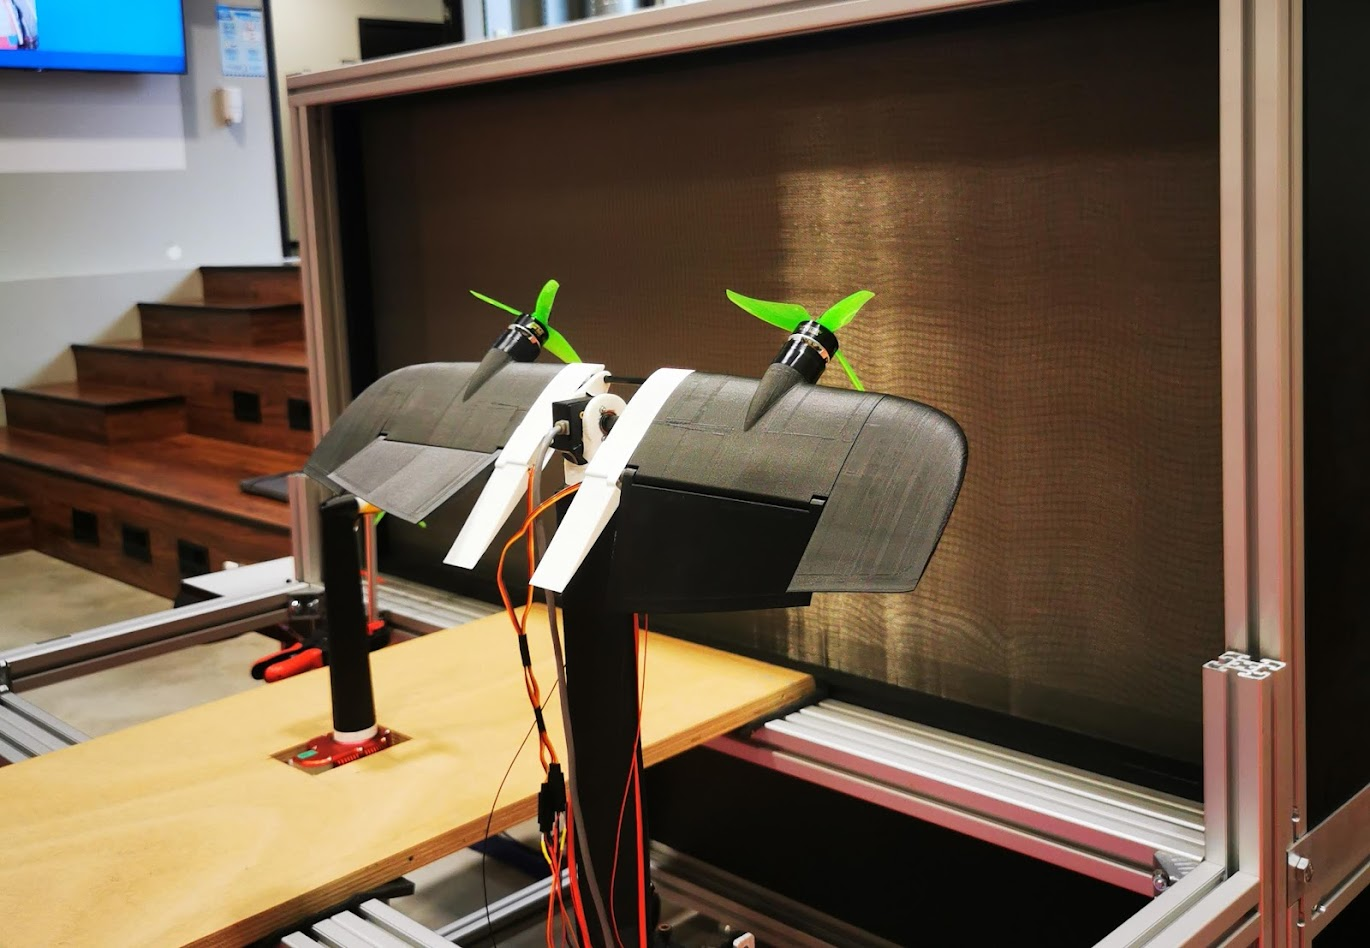
\includegraphics[trim=0cm 5cm 0cm 6cm,clip,width=1\columnwidth]{figures/real_test_bench-min.jpg}
    \caption{Single degree-of-freedom DarkO model in front of the WindShape.}
    \label{fig:real_test_bench}
\end{figure}
The photo reported in Fig. \ref{fig:real_test_bench} shows the experimental device in its test environment. The drone is placed in front of an open wind tunnel, called WindShape, generating a horizontal wind between 2 and 16 \SI{}{\meter\per\second}. Thus, during our tests, we consider the vertical wind component to be zero. The drone is placed at the centre of the WindShape, in the most laminar flow area, while the hot wire sensor is placed as close as possible to the drone. 

The geometry of the experimental setup allows placing the power and signal cables close to the centre of rotation so as to minimize their frictional effects on the structure. Despite this fact, the rotation system inevitably interferes with the drone, by creating parasitic forces, notably drag. The projected surface of the joint is small compared to the wing surface, so that the drag generated by this support is low compared to the drag of the wing and the propellers, thus it can be neglected.
\begin{figure}[!ht]
    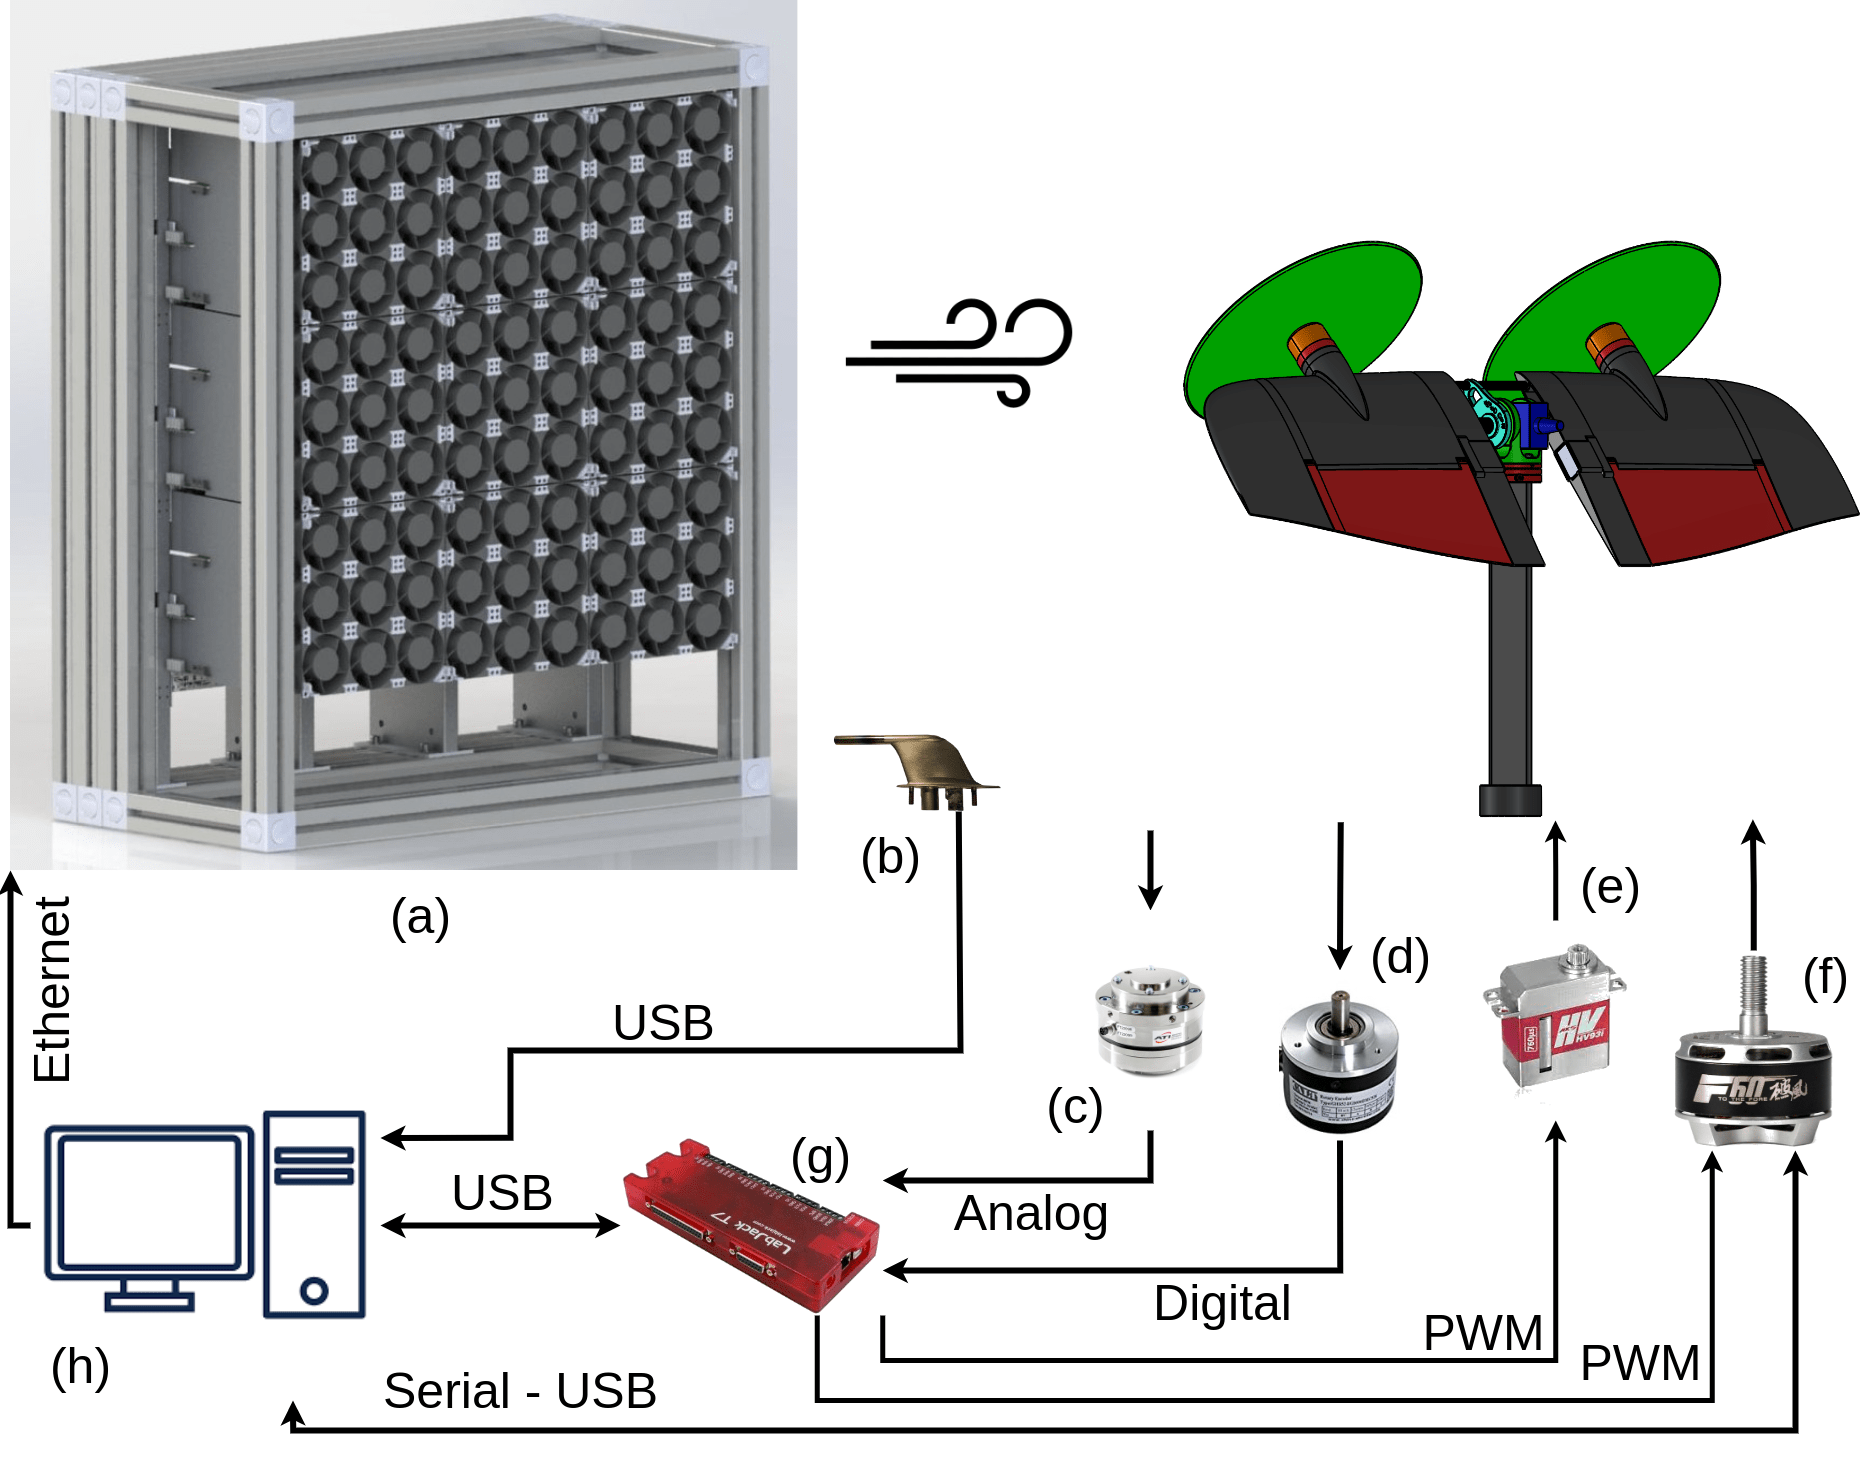
\includegraphics[width=\columnwidth]{figures/maquette-min.png}
    \caption{Virtual flight testing architecture: WindShape (a); Airspeed sensor (b); Force/Torque sensor (c); Rotary encoder (d); Servomotor (e); Brussless motor + ESC (f); LabJack (g); Control computer (h)}
    \label{fig:archi}
\end{figure}

A schematic diagram of the functional subcomponents of the experimental device and their interconnection is shown in Fig. \ref{fig:archi}, which is explained below by referring to the various subsystems with their corresponding letter (a)-(i).

The motors (f) are powered by an external 12v 20Ah battery and the servo motors (e) are powered by 5v via a LabJack T7 \cite[]{LabJack} acquisition module (g). The LabJack module (g) concentrates most of the sensing/actuating signals: six analog inputs for the force/torque sensor (c), two digital quadrature inputs for the rotary encoder (d), one analog input (or serial link depending on the sensor) for the airspeed sensor (b), two digital PWM (Pulse Width Modulation) outputs for the motors (f) and two digital PWM outputs for the servomotors (e). 
%Finally, to measure the propeller's speed, we use the telemetry output of the motor controllers (ESC) (f). Such outputs provide the temperature of the ESCs, the supply voltage, the absorbed current and the speed of rotation of the motors. We retrieve the two telemetries on two serial links at 115200 bauds directly on the control computer by using serial-USB converters, because the LabJack (g) cannot handle such fast communications. It is interesting to note that the telemetry data are not sent continuously by the ESCs, but only as a result of a request sent to the PWM control pin. Therefore, we regularly send a 30µs pulse, to which the ESC responds with a 10 bytes frame containing the above described measurements.
The elevons are driven by servomotors that do not provide a position measurement signal, therefore we use the setpoint, assuming a perfect actuator, which is reasonable, due to the software saturation imposed on the elevons commanded input and the correct sizing of the servomotors with respect to the involved forces.\\
The LabJack  (g)  has an application programming interface (API), allowing for a remote connection with a computer. We have developed a Python code that communicates with the LabJack in order to retrieve the sensor values, compute the command to be applied to the actuators according to the control scheme presented below, and generate the output signals for the actuators. The data collected from the LabJack is recorded to be used for post-processing and generate the plot reported in Section \ref{sec:exp}. \\
To generate the wind, we use a WindShape device, which also has an API, allowing it to be controlled through an Ethernet network. The developed Python code can assign the WindShape wind speed and therefore act on the model. It is thus possible to test a set of hovering configurations and their associated transients in the same test campaign, without any action on the model. 



\subsection{Software-in-the-loop translational motion}
Since the prototype is connected to the fixed support, it is not possible to experimentally reproduce the translational motion.  We have instead included a software-in-the-loop routine that simulates the translational motion by integrating the force measurements available at the joint. In particular, the translational velocity (resp. position) of the UAV is obtained by single (resp. double) integration of the data measured by the force sensor. We neglect the aerodynamic influence of the (simulated) speed on the wing for the sake of simplicity. In particular, from equations (\ref{eq:dyna1}) and (\ref{eq:dyna2}), we obtain the simplified model
\begin{subequations}\label{eq:accel_sensor}
\begin{align}
    \boldsymbol{\dot v} &= \boldsymbol{g} + \frac{1}{m}\left( R(\boldsymbol{q})(F\boldsymbol{u} +  D_{\text{f}}(\delta) R^\top(\boldsymbol{q})\lVert \boldsymbol{w} \rVert \boldsymbol{w}) \right)\\
    &= \boldsymbol{g} + \frac{1}{m} \boldsymbol{F}_{meas} \label{eq:sub_accel_sensor},
\end{align}
\end{subequations}

where $\boldsymbol{F}_{meas}$  represents the forces measured by the sensor in the bias-corrected inertial reference frame. To calibrate the bias correction, at the initialization, the measured forces are averaged over 6000 samples, the model being blocked at a steady position (pitch angle at 0°, namely vertical orientation). Removing the bias from the measured force at each measurement, we subtract the gravity effect on the model from the measurement. An artificial mass $m$ is instead assigned to the software-in-the-loop dynamics according to (\ref{eq:sub_accel_sensor}), which allows testing several configurations to better appreciate the influence of the drone's mass on possible transient saturation events. This allows investigating scenarios involving the nontrivial mass of the battery, which is not present in our model. Although this manipulation is easy, it does not represent perfectly the reality because we do not take into account the distribution of the masses in the drone and thus the inertia modifications.
The transitional velocity and position of the UAV are then obtained by single and double numerical integration of the acceleration as in (\ref{eq:accel_sensor}), using a trapezoidal numerical integration.



\section{Integral-based linear control}\label{sec:3dofcmd}
In our previous work \cite[III.B]{sansouECC} we proposed a proportional feedback stabilizing a hovering position in the absence of wind (perturbation). We propose here an extension including integral action, suitable for operating with a non-measured perturbation represented by a constant wind. The objective is to stabilize the drone at the reference position, rejecting the unknown constant wind disturbance.

\subsection{Description of the control scheme}
We experiment the situation with the wind only acting along the $x_{[I]}$ axis, with the drone oriented towards the wind, i.e. with zero roll and yaw angles. In this configuration, the wind only acts on the linear velocity along the $x_{[B]}$ and $z_{[B]}$ axes, and it only generates a moment about the $y_{[B]}$ axis. A careful inspection of the control and the disturbance input matrices $F$, $M$ 
in \eqref{eq:FandM} suggests an effective control architecture to reject a constant disturbance. Indeed, the ailerons and the propellers can be used symmetrically to generate respectively a moment about the $y_{[B]}$ axis and a force along the $x_{[B]}$ axis, thus compensating the disturbance effect. Nevertheless, there is still a force along the $z_{[B]}$ axis to be compensated, and an integral action can asymptotically converge to the desired force, even with a non-measured wind disturbance $w$. We may thus stabilize the UAV at a hovering position, different from the zero-wind equilibrium. The control solution exploits the pitch angle degree of freedom, for compensating the wind effect.
\begin{figure}[ht!]
    \centering
    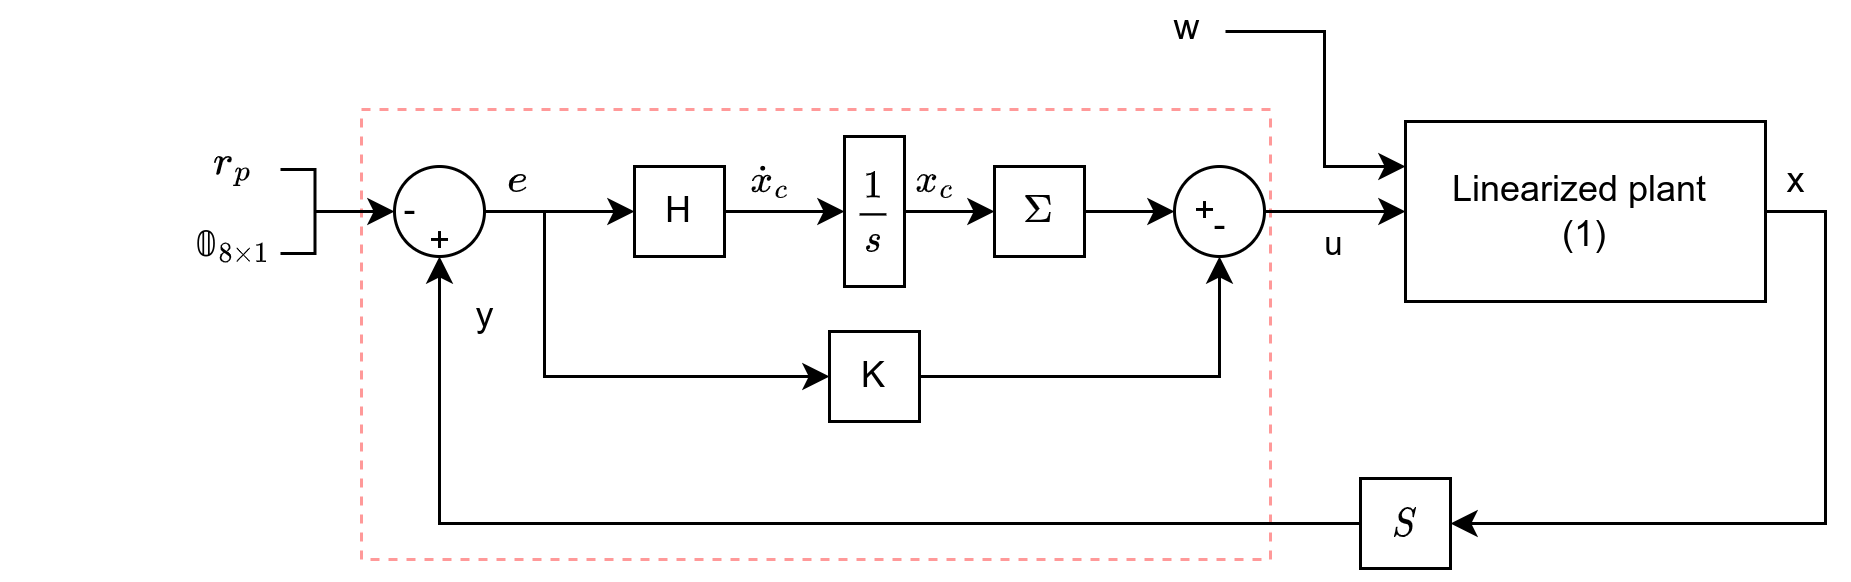
\includegraphics[trim=5cm 0cm 0cm 0cm,clip,width=1\columnwidth]{figures/commande_integrale_ACA-min.png}
    \caption{Proposed integral-based controller.}
    \label{fig:commande_int}
\end{figure}\\
The proposed controller, shown in Fig. \ref{fig:commande_int},  corresponds to 
\begin{minipage}[t]{0.58\columnwidth}
    \begin{align}
        \dot{x_{c}} &= H(y-\begin{bmatrix}r_{p}\\\mathbb{0}_{8\times 1} \end{bmatrix}),\\
        y &= S x,\\
        u &= \Sigma x_{c} + K(y-\begin{bmatrix}r_{p}\\\mathbb{0}_{8\times 1} \end{bmatrix}),
    \end{align}
\end{minipage}
\begin{minipage}[t]{0.42\columnwidth}
    \begin{align}
        S =\begin{bmatrix} \mathbb{I}_{7} &  \mathbb{0}_{7\times 5} \\
         \mathbb{0}_{4\times 8} &  \mathbb{I}_{4}
          \end{bmatrix}, 
    \end{align}
    \begin{align}
        \Sigma = \begin{bmatrix} 1 & 1 & 0 & 0\\ 0 & 0 & 1 & 1\end{bmatrix}^\top,
    \end{align}
\end{minipage}

where $x_{c} \in \mathbb{R}^{2}$ is the integrator state; $r_{p} \in \mathbb{R}^{3}$ is the constant reference comprising a target position for the translational motion; $S$ is an output selection matrix, which removes the pitch angle component from the measured output (impacting only the quaternion linearization) to form $y$; $\Sigma$ is an input allocation matrix that allows assigning the first component of the integrator state to the motor control and the second component to the elevon control. $K$, $H$ are constant stabilizing gains to be selected in such a way that the linear closed loop matrix 
\begin{align} \label{eq:close_matrix}
    \begin{gathered}
        A_{cl} \!= \!
        \begin{bmatrix}A & \mathbb{0}_{12\times 2} \\ HS & \mathbb{0}_{2\times 2}\end{bmatrix} \!- \!\begin{bmatrix}G \\ \mathbb{0}_{2\times 4}\end{bmatrix} \left( K \begin{bmatrix}S & \mathbb{0}_{11\times 2}\end{bmatrix} -  \begin{bmatrix}\mathbb{0}_{4\times 12} & \Sigma \end{bmatrix}\right),
    \end{gathered}
\end{align}
characterizing the linearized closed loop be Hurwitz, to ensure stabilization with the linearized dynamics related to the zero-wind scenario \eqref{eq:linearized}.

In a nutshell, matrix (\ref{eq:close_matrix}), describes the closed loop shown in Fig. \ref{fig:commande_int}: an output feedback with 11 outputs, consisting of the three positions, the three linear velocities, two out of three angles ($\phi$ and $\psi$) and the three angular velocities. This structure can be seen as a MIMO proportional-integral solution resulting from a careful observation of the UAV linearized dynamics, which allows a minimal number of integrators embedded in the controller. This control should allow constant disturbances rejection while having a satisfactory robustness. The gain $K$ corresponds to the proportional  term and the gain $H$ weights the integral term, inducing convergence to the target. The allocation matrix $\Sigma$ leads to a symmetrical use of the propellers and ailerons. We must then tune $K$ and $H$ to obtain a satisfactory trade-off between robustness and disturbance rejection. We implement a multi-objective synthesis based on an $H_{\infty}$ optimization method, described next.

\subsection{\texorpdfstring{$H_{\infty}$}{H {infty}}-based optimization} \label{sec:h_inf}

To perform a robust selection of $K$ and $H$, we first characterize several transfers functions in Fig. \ref{fig:commande_int}.
%To perform a robust selection of $K$ and $H$ we represent the scheme of Fig. \ref{fig:commande_int}
%in the compact form of Fig. \ref{fig:lft}, where the augmented plant includes both the integral action and dynamics (\ref{eq:dyna_simp}). 
The measurement output $y$ is used for feedback, the input $u$ is the sum of the integral input $\Sigma x_{c}$ and the proportional action $K e$. The output $z$ corresponds to the output performance signals to control ($e$, $w$, $u$, $y$, $r_{p}$). Thanks to weighting functions $W=\diag (W_{1},..., W_{4})$, the design of $H$ and $K$ aims to reject a low frequency perturbation or step $w$ acting on $y$. In short, the design goal is to bring $y$ to zero despite the low frequency disturbance on $w$. 

From the Nyquist criterion, we know that the margin corresponds to the minimal distance between the singularity (real point -1) and the product between the controller (C) and the plant (P). Consequently, we define the input modulus margin as $MM_{u} =\min_{\omega\in R}|1-CP|$ and the output modulus margin as $MM_{y} =\min_{\omega\in R}| 1-PC |$ for a positive feedback. We first introduce the output sensitivity function  $T_{r \rightarrow \epsilon}=S_{y}=(1-PC)^{-1}$, so that $\lVert S_{y} \rVert_{\infty}=MM_{y}^{-1}$ and the input sensitivity function $T_{d \rightarrow u}=S_{u}=(1-CP)^{-1}$, so that $\lVert S_{u} \rVert_{\infty}=MM_{u}^{-1}$. Consequently, the minimization of the  $H_{\infty}$-norm of $S_{u}$ or $S_{y}$, leads to improving the input and output modulus margins. As our system is MIMO, we give importance to both the input and output sensitivity functions, because they do not commute. We also define the transfer functions $T_{r \rightarrow u}= CS_{y} = S_{u}C$ and $T_{w \rightarrow y}$. In order to guarantee a satisfactory trade-off between robustness and performance, we select the weighting functions $W_{1}$, $W_{2}$, $W_{3}$ and $W_{4}$ linked to $\lVert W_{1} T_{r \rightarrow \epsilon}(s)\rVert_{\infty} \leq 1 $ and $\lVert W_{2} T_{d \rightarrow u}(s)\rVert_{\infty} \leq 1 $, corresponding to robustness margins at the inputs and outputs, $\lVert W_{3} T_{r \rightarrow u}(s)\rVert_{\infty} \leq 1 $ limiting the control effort, $\lVert W_{4} T_{w \rightarrow y}(s)\rVert_{\infty} \leq 1 $ ensuring suitable wind disturbance rejection. Specifically, the weighting functions are tuned as
\begin{align} \label{eq:weight_gain}
    &W_{1} =  0.5, \quad
    W_{2} = 0.5, \quad
    W_{3} = 0.8, 
    &W_{4} = 0.5.
\end{align}
The values of $W_{1}$ and $W_{2}$ ensure $MM_{u} >  6~dB$ and $MM_{y} >  6~dB$, $ W_{3}$ and $W_{4}$ are tuned to obtain a satisfactory trade-off between the different specifications. The weight $ W_{4} $  allows managing, among other things, the speed of the rejection.
% \begin{figure}[ht!]
%     \centering
%     \includegraphics[width=0.9\columnwidth]{picture/Copie de lft.png}
%     \caption{$H_{\infty}$-oriented plant-controller feedback representation.}
%     \label{fig:lft}
% \end{figure}

% With these selections, we cast the design problem for $K$ and $H$ as a generalized mixed sensitivity problem providing good input and output specifications for the closed loop
With selections \eqref{eq:weight_gain}, we cast the design problem for $K$ and $H$ as an $H_{\infty}$ synthesis under order constraint, providing good input and output specifications for the closed loop:
\begin{align*} \label{eq:pb_optim}
&\min_{C}\quad \begin{Vmatrix}
    W_{1} T_{r \rightarrow \epsilon}(P,C)\\
    W_{2} T_{d \rightarrow u}(P,C)\\
    W_{3} T_{r \rightarrow u}(P,C)\\
    W_{4} T_{w \rightarrow y}(P,C)
    \end{Vmatrix}_{\infty}, \text{ subject to} \\ &C \in \mathbb{R}^{11 \times 4} \text{ stabilizes } P \text{ internally,} \numberthis
\end{align*}

where $P$ is the augmented plant containing the integral action and the linearized UAV dynamics. In addition, we impose constraints on the gains $K$ and $H$ ensuring that the closed loop with experimental device only evolves in the ($x$,$z$) plane, compatibly.


We solved (\ref{eq:pb_optim}) using Systune \cite[]{1576856}. Based on non-smooth optimization, Systune dealing with several non-convex scenarios, such as the structured control architecture where we optimize the gain matrices $K$, $H$. The optimization algorithm returns optimized selections of 
\begin{align}\label{eq:HK}
\begin{bmatrix}
H\\ \hline K 
\end{bmatrix} = \smallmat{
\shortminus1.902 & 0 & 7.201 & \shortminus9.043  & 0 & 33.244 & 0 & 0 & 0 & 4.696  & 0 \\ 
0.425 & 0 & \shortminus1.620 & 2.024  & 0 & \shortminus7.480 & 0 & 0 & 0 & \shortminus1.045  & 0 \\  \hline
0.035 & 0 & \shortminus0.728 & \shortminus1.853  & 0 & \shortminus4.445 & 0 & 0 & 0 & \shortminus0.323  & 0 \\ 
0.035 & 0 & \shortminus0.728 & \shortminus1.853  & 0 & \shortminus4.445 & 0 & 0 & 0 & \shortminus0.323  & 0 \\ 
0.217  & 0 & \shortminus0.164  & 1.074 & 0 & \shortminus0.527 & 0 & 0 & 0 & \shortminus0.773 & 0 \\ 
0.217  & 0 & \shortminus0.164  & 1.074 & 0 & \shortminus0.527 & 0 & 0 & 0 & \shortminus0.773 & 0  
}
\end{align}
Introducing a closed-loop spectral abscissa $\alpha = -0.2381$ for $A_{cl}$ in (\ref{eq:close_matrix}).

\section{Résultats}






